%!TEX program = xelatex
\documentclass[12pt,a4paper]{article}

\usepackage{cite}
\usepackage{xltxtra}
%%% Математические пакеты %%%
\usepackage{amsthm,amsfonts, amssymb,amscd}  % Математические дополнения от AMS
\usepackage{amsmath}
\usepackage{mathtools}
\usepackage{unicode-math}
%%% Кодировки и шрифты %%%
 \usepackage{polyglossia}                          % Поддержка многоязычности
\usepackage{fontspec}
\usepackage{xunicode}

%%% Общее форматирование
\usepackage[singlelinecheck=off,center]{caption}    % Многострочные подписи
\usepackage{soul}                                   % Поддержка переносоустойчивых подчёркиваний и зачёркиваний
\usepackage{icomma}                                 % Запятая в десятичных дробях
%%% Оформление абзацев %%%
\usepackage{indentfirst}     

\usepackage{xcolor}

\usepackage[nodayofweek]{datetime}
%\usepackage{fancyhdr}
\usepackage{hyperref}

        % Подключаемые пакеты
% \defaultfontfeatures{Ligatures={TeX},Renderer=Basic}  %% свойства шрифтов по умолчанию
% \setmainfont[Ligatures={TeX,Historic}]{Times New Roman} %% задаёт основной шрифт документа
% \setmainfont[Ligatures={TeX}]{Times New Roman} %% задаёт основной шрифт документа
% \setsansfont{Helvetica}                    %% задаёт шрифт без засечек
% \setsansfont{CMU Serif}
% \setmonofont{American Typewriter}               %% задаёт моноширинный шрифт
% \setmathrm{xits-math.otf}
% \setmathfont{xits-math.otf}
\ifxetex
\defaultfontfeatures{Ligatures={TeX},Renderer=Basic}
\setromanfont[Ligatures={TeX,Historic}]{Times New Roman}
\setsansfont[Ligatures={TeX,Historic}]{Arial}
\newfontfamily\cyrillicfont{Arial}
\setmainfont[Ligatures={TeX,Historic}]{Times New Roman}
\newfontfamily\cyrillicfont{Times New Roman}
\setmonofont[Color={0019D4}]{Courier New}
\newfontfamily{\cyrillicfonttt}{Courier New}
%%% Кодировки и шрифты %%%
\setdefaultlanguage{russian}  %% устанавливает главный язык документа
\setotherlanguage{english}
\else
\fi

\usepackage[left=2cm,right=2cm,top=2cm,bottom=2cm]{geometry}
\parindent=1cm
          % Пользовательские стили

\newcommand{\then}{\ \Longrightarrow \ }
\newcommand{\eps}{\varepsilon}
\newcommand{\com}{\backslash \backslash}
\renewcommand{\C}{\mathbb{C}}
\newcommand{\R}{\mathbb{R}}
\newcommand{\Q}{\mathbb{Q}}
\newcommand{\Z}{\mathbb{Z}}
\newcommand{\N}{\mathbb{N}}
\newcommand{\vphi}{\varphi}
\newcommand{\iaoi}{\ \Longleftrightarrow \ }
\newcommand{\empt}{\varnothing}
\newcommand{\A}{\mathfrak{A}}
\newcommand{\sm}{\sum\limits}
\newcommand{\I}{\mathbb{I}}
\renewcommand{\it}{\int\limits}
\renewcommand{\L}{\mathcal{L}}
\renewcommand{\bar}{\overline}
\renewcommand{\tilde}{\widetilde}

\newtheorem*{thmnn}{Теорема}
\newtheorem*{thm}{Теорема}
\newtheorem*{dfn}{Определение}
\newtheorem*{sug}{Предложение}
\newtheorem*{prop}{Свойство}
\newtheorem*{lem}{Лемма}
\newtheorem*{con}{Следствие}
\newtheorem*{note}{Замечание}
\newtheorem{exer}{Задача}
\newtheorem*{notation}{Напоминание}
\newtheorem*{ex}{Пример}
\newtheorem*{design}{Обозначение}

\ifxetex 
\newcommand{\mathbbold}{\mathbb}
\else
\DeclareMathAlphabet{\mathbbold}{U}{bbold}{m}{n}
\fi

\DeclareMathOperator{\ord}{ord}
\DeclareMathOperator{\val}{val}
\DeclareMathOperator{\rk}{rk}
\DeclareMathOperator{\cov}{cov}
\DeclareMathOperator{\cor}{cor}
\DeclareMathOperator{\diag}{diag}

\DeclareMathOperator*{\argmin}{arg\,min}
\DeclareMathOperator*{\argmax}{arg\,max}

% \ifdef\T {
%     \renewcommand{\T}{\mathrm{T}}
% } {
%     % \DeclareMathOperator*{\T}{\mathrm T}
%     \newcommand{\T}{\mathrm{T}}
% }

\newcommand{\Tr}[1]{#1^{\mathrm{T}}}


\newcommand{\Inner}[2]{\langle\,#1, #2\,\rangle}

\newcommand{\Outer}[2]{ #1\otimes#2}  

\newcommand{\Header}{
  \pagestyle{empty}
  \begin{center}
    {\Large\bf 
     Ответы к коллоквиуму по Многомерному Анализу Данных 
     }\\
    \vspace{0.7em}
    {Собрано {\today} в {\currenttime}}
  \end{center}

  \vspace{1em}
  \tableofcontents
  \pagebreak
}


\begin{document}
    \Header{}
    \subsection{Билет 1. Многомерное нормальное распределение. Вектор мат.ож. и ковар.матрица при лин. преобразовании (умножении на матрицу).}
\paragraph{Нормальное распределение}
\begin{dfn}
    \label{dfn::1::mnd1}
    %Пусть $\mu \in \mathbb R^p$ и $\Sigma \in \mathrm M_{p, p}(\mathbb R)$ 
    Говорят, что случайный вектор $\mathbb \xi = (\xi_1, \xi_2, \ldots, \xi_p)^\mathrm T$ имеет $p$-мерное нормальное распределение, если %$\mathcal N(\mu, \Sigma)$, если 
    для любых $\{a_i\}_{i=1}^p \subset \mathbb R$ линейная комбинация $\sum_{i=1}^p a_i \xi_i$ имеет 
    нормальное распределение.\footnote{Здесь распределение Дирака тоже считаем нормальным.}
    Если обозначить $\mu = \mathbb E \xi$, $\Sigma = \mathrm{Cov} \xi$, то пишут $\xi \sim \mathcal N(\mu, \Sigma)$.
\end{dfn}
\begin{thm}
    \label{thm::1::mnd2}
    Пусть $\mu \in \mathbb R^p$ и $\Sigma \in \mathrm M_{p, p}(\mathbb R)$ --- невырожденная матрица.
    Рассмотрим случайный вектор $\mathbb \xi \sim \mathcal N(\mu, \Sigma)$.
    Тогда $\mathbb \xi$ имеет плотность:
    \begin{gather}
        \label{mnd_dens}
        p_\mathbb \xi (\mathbf x) = \frac{1}{(2 \pi)^{p/2} \sqrt{\det \Sigma}}
        e^{-\frac{1}{2} (\mathbf{x} - \mu)^\mathrm T \Sigma^{-1} (\mathbf x - \mu)},
    \end{gather}
    для любого $\mathbf x \in \mathbb R^p$.\footnote{Убедитесь, что при $p = 1$ получается одномерная плотность.}
\end{thm}

Заметим, что в определении \ref{dfn::1::mnd1} не требуется невырожденность ковариационной матрицы $\Sigma$.
Если же $\Sigma$ вырожденная, то это означает, что распределение сосредоточено на подпространстве в $\mathbb R^p$.\footnote{Чтобы
    это осознать, представьте себе $\eta \sim \mathcal N(0, 1)$. На каком подпространстве (и как) распределен вектор $(\eta, 0)^\mathrm T$?
}
\paragraph{Линейное преобразование}
\begin{thm}
Пусть $\xi \sim \mathcal N(\mu, \Sigma)$, где $\mu \in \mathbb R^p$, а $\Sigma \in \mathrm M_{p,p}(\mathbb R)$. Рассмотрим матрицу $\mathbb A \in \mathrm M_{d,p}(\mathbb R)$.
    Тогда $\mathbb A \xi \sim \mathcal N\left(\mathbb A \mu, \mathbb A \Sigma \mathbb A^\mathrm T\right)$.  \end{thm}
\begin{proof}
    Утверждение следует из линейности мат. ожидания и того, что $\mathrm{Cov}(\xi) = \mathbb E(\xi-\mathbb E\xi)(\xi-\mathbb E\xi)^\mathrm T$.\footnote{В
    одномерном случае это должно совпасть с обычным определением ковариации.}
\end{proof}

\subsection{Билет 2. Оценки вектора средних и ковар.матрицы. Несмещенная оценка ковар. матрицы.}
\paragraph{Генеральный язык.}

Пусть дан вектор $\xi = (\xi_1, \ldots, \xi_p)^\mathrm T$. Вектором средних называется $\mathbb E\xi = (\mathbb E\xi_1, \ldots, \mathbb E\xi_n)^\mathrm T$.
Ковариационная матрица --- $\mathrm{Cov}(\xi) = \mathbb E(\xi-\mathbb E\xi)(\xi-\mathbb E\xi)^\mathrm T$.
\paragraph{Выборочный язык.}

Генеральную совокупность обозначим $\xi$.
Рассмотрим $\mathbb X = [X_1\colon\ldots\colon X_p] \in M_{n, p} (\mathbb R)$ --- матрица данных. $X_i$ --- $i$-тый признак. 
Тогда $\widehat{\mathbb E \xi} = \left(\overline X_1, \ldots, \overline X_p\right)$.

Введем $X_i^{(c)}$--$i$-тый центрированный признак и рассмотрим $\mathbb X^{(c)} = [X_1^{(c)}, \ldots, X_p^{(c)}]$ --- матрицу центрированных данных.
Тогда $\widehat{\mathrm {Cov}(\xi)} = {\mathbb X^{(c)}}^\mathrm T \mathbb X^{(c)} / n$. В несмещенной оценке ковариационной матрицы знаменатель дроби равен $n-1$.

\textit{Здесь также нужно провести доказательство для дисперсии, что несмещенная оценка является несмещенной. Думаю, что все это уже хорошо умееют делать.}

\subsection{Билет 3. Распределение вектора средних}
\begin{thm}
    Пусть дана выборка (на априорном языке) $\mathbf x_1, \ldots, \mathbf x_n \ldots$ c ковариационной матрицей $\Sigma$.
    Обозначим $\overline{\mathbf x}_n$ --- выборочное среднее первых $n$ индивидов.
    Тогда для выборочного среднего имеет место следующая (слабая) сходимость:
    \begin{gather*}
        \sqrt{n} (\overline{\mathbf x}_n - \mu) \to \mathcal N(\mathbbold{0}, \Sigma).
    \end{gather*}

    Если же $\mathbf x_1, \ldots, \mathbf x_n \sim \mathcal N(\mu, \Sigma)$, то выборочное среднее $\overline{\mathbf x}_n$ имеет распределение $\mathcal N(\mu, \Sigma/n)$.
\end{thm}

Заметим, что асимптотическая сходимость есть ни что иное, как многомерное обобщение ЦПТ в форме Леви. Все могут вывести из этого обобщения обычную (одномерную) теорему?

\subsection{Билет 4. Переход к новым признакам с помощью ортогональной матрицы. Пример про способности по математике и физике (выписать матрицу вращения)}

\paragraph{Переход к новым признакам.}
Рассмотрим случайный вектор $\xi \in \mathbb R^p$ и детерминированный вектор $a \in \mathbb R^p$.
Если $\xi$ рассматривать как набор из $p$ признаков, то $\eta = a^\mathrm T \xi$ --- новый признак.

Рассмотрим же теперь матрицу $\mathbb A = [A_1 \colon \ldots \colon A_d] \in \mathrm M_{p, d}(\mathbb R)$. Тогда $\mathbb A^\mathrm T \xi$ --- набор из новых $d$ признаков.

На выборочном языке то же самое перепишется так:
$Z = \mathbb X a$ --- для одного признака и $\mathbb Z = [Z_1 \colon \ldots \colon Z_d] = \mathbb {X A} \in \mathrm M_{n, d}(\mathbb R)$ --- для $d$ признаков.
Заметим, что в последней записи новыми признакими как раз будут являться столбцы $Z_1, \ldots, Z_d$.

\paragraph{Факторы и факторные нагрузки.}
Пусть задана матрица данных $\mathbb X = [X_1 \colon \ldots \colon X_p] \in \mathrm M_{n, p}(\mathbb R)$. Обозначим $d = \mathrm{rk} (\mathbb X)$.
Перейдем с помощью матрицы $\mathbb A$ к $d$ ортогональным признакам $\{Z_i\}_{i=1}^d$.
Формально, это означает, что $\mathbb Z = \mathbb {X A}$, где $\mathbb Z = [Z_1 \colon \ldots \colon Z_d]$ и $Z_i \perp Z_j$ при $i \neq j$.
С точки зрения линейной алгебры $\{Z_i\}_{i=1}^d$ образуют ортогональный базис в пространстве признаков\footnote{Формально, $\mathrm {span} (X_1, \ldots X_p)$.}.

Превратим этот базис в ортогональный: для всех $i \in 1:d$ положим $Q_i = Z_i / \|Z_i\|$.
Таким образом, $\{Q_i\}_{i=1}^d$ --- ОН-базис в пространстве признаков.
Введем матрицу $\mathbb Q = [Q_1 \colon \ldots \colon Q_d] \in \mathbb M_{n,d}(\mathbb R)$.

Разложим исходные признаки по ОН-базису, то есть по всем $j \in 1:p$
\begin{gather*}
    X_j = \sum_{k=1}^d f_{jk} Q_k,
\end{gather*}
где $f_{jk} = (X_j, Q_k)$ для всех $j \in 1:p$ и $k \in 1:d$.
Введем матрицу $\mathbb F = [F_1 \colon \ldots \colon F_d]$, где $\left(F_j\right)_i = f_{ij}$. Вектора $Q_\cdot$ называют \textit{факторами},
а $f_{\cdot \cdot}$ --- \textit{факторными нагрузками}.
Тогда ясно, что $F_k = \mathbb X^\mathrm T Q_k \in \mathbb R^p$\footnote{Чтобы не запутаться, где тут транспонирование есть один простой трюк.
    Помните, что вы работаете с признаками! Это же точно столбцы матрицы $\mathbb X$. Интерпретируйте алгебраические преобразования именно как преобразования над
    признаками. Для формальной проверки достаточно обычно проверить, сходятся ли размерности.}.
    Но $\mathbb X = \sum_{k=1}^d Q_k (\mathbb X^T Q_k)^\mathrm T$\footnote{Просто разложили элементы пространства по базису, правда?}.
Следовательно, $\mathbb X = \mathbb Q \mathbb F^\mathrm T$.

\paragraph{Разложение с помощью ортогональных признаков.}
Итак получено разложение $\mathbb X = \mathbb Q \mathbb F^\mathrm T$, при этом $\mathbb Q^\mathrm T \mathbb Q$ --- единичная матрица порядка $d$.\footnote{Заметим,
    что $\mathbb Q \mathbb Q^\mathrm T$ не обязано совпадать с единичной матрицей. Разве это удивительно? Вновь, используем язык признаков.
    Лишь одно из перемножений имеет интерпретируемый смысл.}
В этом разложении лишь $Q$ задает ОН-базис. Система, заданная столбцами матрицы $\mathbb F$ совершенно не обязана быть нормированной.
Рассмотрим $P_j = F_j / \|F_j\|$ и положим $\sigma_j = \|F_j\|$. Введем матрицы $\Sigma = \mathrm {diag} (\sigma_1, \sigma_2, \ldots, \sigma_d)$ и
$\mathbb P = [P_1 \colon \ldots \colon P_d] \in \mathrm M_{n, d}(\mathbb R)$.
Тогда $\Sigma \mathbb P^\mathrm T = \mathbb F^\mathrm T$.\footnote{Смотрим на это на языке столбцов. Тогда все станет ясно.} 
А значит $\mathbb X = \mathbb Q \Sigma \mathbb P^\mathrm T$.

C другой стороны, было показано, что $\mathbb X = \sum_{i=1}^d Q_i F_i^\mathrm T = \sum_{i=1}^d \sigma_i Q_i P_i^\mathrm T$.

\bigskip

Обратим внимание, что в получившемся разложении $P_i$, обычно\footnote{\color{blue} Я тут сам не понимаю --- вроде бы в общем случае линейной независимости не от куда взяться}
не являются ортогональными, а лишь линейно-независимыми. В дальнейшем, утверждается, что единственным биортогональным разложением (то есть таким, когда $P_i$ ортогональны) является SVD.

\begin{ex}
    Пусть число признаков $p = 2$, то есть $\mathbb X = [X_1 \colon X_2]$. При этом $X_1$ показывает количество баллов по математике, а $X_2$ --- количество баллов по физике.
    Рассмотрим матрицу поворота:
    \begin{gather*}
        \mathbb A = \frac{1}{\sqrt{2}}
        \begin{pmatrix}
            1  &  1 \\
            1  & -1
        \end{pmatrix}.
    \end{gather*}
    Рассмотрим два новых признака $\mathbb Z = [Z_1 \colon Z_2] = \mathbb {X A}$, где $Z_1 = (X_1 + X_2) / \sqrt{2}$ --- отражает общие способности, $Z_2 = (X_1 - X_2) / \sqrt{2}$ --- ``разница'' между способностями по математике и физике.
    Очень рекомендуется выписать все буковки, которые встречались раньше в этом примере (в частности, матрицу факторных нагрузок).
\end{ex}


\subsection{Билет 5. Разложение матрицы данных при переходе к новым признакам в виде суммы и в матричном виде}

См. предыдущий билет. По всей видимости интересует представление в виде $\mathbb X = \mathbb Q \mathbb F^\mathrm T$.
Заметим, что справедливо представление $\mathbb X = \sum_{k=1}^d Q_k F_k^\mathrm T$.
Определим $\mathbb X_k = Q_k F_k^\mathrm T$ для $k \in 1:d$. Ясно, что $\mathrm{rk}(X_k) = 1$.\footnote{Почему все строки (или все столбцы) этой матрицы линейно зависимы?}
Тогда $\mathbb X = \sum_{k=1}^d \mathbb X_k$.

\subsection{Билет 6. Как определяется вклад новых признаков}

\begin{dfn}
    Зафиксируем $t, s \in \mathbb N$ (абстрактные). На пространстве $\mathrm M_{t,s} (\mathbb R)$ введем \textit{фробениусово}
    скалярное произведение: для любых матриц $\mathbb X = \{x_{ij}\}, \mathbb Y = \{y_{ij}\} \in \mathrm M_{t, s} (\mathbb R)$ определим $(\mathbb X, \mathbb Y)_F = \sum_{i,j} x_{ij} y_{ij}$.\footnote{
    Несложно проверить, что это, действительно, скалярное произведение.}.

    Это скалярное произведение порождает \textit{фробениусову} норму матрицы: \\$\|\mathbb X\| = \sqrt{\sum_{i,j} x_{ij}^2}$\footnote{Кто помнит, кажется, 5тую главу вычей второго курса,
    знает, что это не самая классная норма, потому что она не подчинена никакой векторной, но для наших целей подходит.}.
\end{dfn}


Вернемся к матрицам $\mathbb X_k$ (cм. билет 5). Если $\mathbb X_i \perp \mathbb X_j$ для неравных $i, j$, то $\mathbb \|X\|^2 = \sum_{k=1}^d \|X_k\|^2$\footnote{Это
стандартное свойство нормы в гильбертовом пространстве.}.
Определим вклад $i$-того признака как отношение $\| \mathbb X_i \|^2 / \| \mathbb X \|^2$.

\begin{lem}
    Пусть $Q_1, Q_2 \in \mathbb R^n$, а $F_1, F_2 \in \mathbb R^p$\footnote{Обозначения выбраны так, чтобы было ясно видно, причем тут матрицы $\mathbb X_k$.}.
    \begin{gather*}
        \left(Q_1 F_1^\mathrm T, Q_2 F_2^\mathrm T\right)_F = (Q_1, Q_2) (F_1, F_2).
    \end{gather*}
\end{lem}
Доказательство леммы проводится очень просто, если записать поэлементно, что происходит.

Из этой леммы следует, что для того, чтобы понятие вклада признака имело смысл (то есть чтобы матрицы $\mathbb X_k$ были ортогональны) достаточно ортогональности новых признаков $Q_i$.

\subsection{Билет 7. Сингулярное разложение, как строится}

Пусть дана матрица $\mathbb Y \in \mathrm M_{L, K}(\mathbb R)$, где $L < K$\footnote{Обозначения здесь вводятся с расчетом на Гусеницу в следующем семестре}.
Рассмотрим матрицу $\mathbb S = \mathbb Y\mathbb Y^\mathrm T \in \mathrm M_{L,L}(\mathbb R)$\footnote{Матрица потом будет обозначать ковариационную, поэтому обозначение правильно ее напоминает.}.
Эта матрица неотрицательно определена и симметрична. Упорядочим ее собственные числа по невозрастанию: $\lambda_1 \geqslant \lambda_2 \geqslant \ldots \geqslant \lambda_L \geqslant 0$.
Обозначим $U_i$ --- нормированный собственный вектор соответствующий собственному числу $\lambda_i$ матрицы $\mathbb S$ (по всем $i \in 1:L$).
Набор $\{U_i\}_{i=1}^L$ образует ОН-базис в $\mathbb R^L$.

Следующее утверждение содержит несколько известных фактов из линейной алгебры (доказывать на коллоквиуме их не нужно).
\begin{thm}
    Обозначим $d = \mathrm {rk}(\mathbb S)$\footnote{Именно новое количество признаков всегда записывалось $d$.}.
    \begin{enumerate}
        \item $d \leqslant{L, K}$.
        \item $d = \mathrm{rk}(\mathbb Y \mathbb Y^\mathrm T) = \mathrm{rk}(\mathbb Y^\mathrm T \mathbb Y) = \mathrm{colrank}(\mathbb Y) = \mathrm{rowrank}(\mathbb Y).$
        \item $\lambda_d > 0$, $\lambda_{d + 1} = 0$.
        \item $\{U_i\}_{i=1}^d$ --- образует ОН-базис в $\mathrm{colspan}(\mathbb Y)$.
    \end{enumerate}
\end{thm}

Следующая теорема играет ключевую роль в первой части.
\begin{thm}[The SVD]
    Введем вектора $V_i = \mathbb Y^\mathrm T U_i / \sqrt{\lambda_i}$ для $i \leqslant d$. 
    \begin{enumerate}
        \item $\{V_i\}_{i = 1}^d$ --- образуют ОН-базис в $\mathrm{rowspan}(\mathbb Y)$. При этом $\mathbb Y^\mathrm T U_i = \mathbbold{0}$\footnote{\color{blue} Кто-нибудь умеет аккуратно это доказывать?}.
        \item $V_i$ --- собственный вектор матрицы $\mathbb Y^\mathrm T \mathbb Y$, соответствующий собственному числу $\lambda_i$ (для $i \in 1:d$).
              Все остальные собственные вектора соответствуют нулевым собственным числам.
        \item $U_i = \mathbb Y V_i / \sqrt{\lambda_i}$ для $i \leqslant d$.
        \item $\mathbb Y = \sum_{k = 1}^d \sqrt{\lambda_i} U_i V_i^\mathrm T$ --- The SVD (Singular Value Decomposition, сингулярное разложение). Терминология: $\sqrt{\lambda_i}$ --- сингулярные числа матрицы $Y$,
              $U_i$ --- левые сингулярные вектора матрицы $\mathbb Y$, $V_i$ --- правые сингулярные вектора матрицы $\mathbb Y$.
    \end{enumerate}
\end{thm}

\begin{proof}
    \begin{enumerate}
        \item Пусть $1 \leqslant i, j \leqslant d$. Тогда $(V_i, V_j) = \left(\mathbb Y^\mathrm T U_i, \mathbb Y^\mathrm T U_j\right) / \sqrt{\lambda_i \lambda_j}= \\ =
              \left(U_i, \mathbb Y \mathbb Y^\mathrm T U_j\right) = \lambda_j (U_i, U_j) \sqrt{\lambda_i \lambda_j} = \delta_{i,j}$.
        \item То, что $V_i$ --- собственный вектор, соответствующий $\lambda_i$ при $i \leqslant d$ проверяется непосредственно. Докажем, что
              $V_i$ при $i > d$ соответствуют нулевым собственным числам. Действительно, пусть некоторый вектор $V$ такой, что $V \perp V_i$ для всех $i \leqslant d$.
              Это означает, что $0 = (\mathbb Y^\mathrm T U_i, V) = (U_i, \mathbb Y U)$ для всех $i \in 1:d$, то есть $\mathbb Y V$ соответствует нулевому собственному числу матрицы $\mathbb Y \mathbb Y^\mathrm T$,
              а значит по первому пункту\footnote{\color{blue} Здесь пока непонятно.}
              $\mathbb Y^\mathrm T (\mathbb Y V) =0$.
        \item Подставьте и все будет хорошо.
        \item Внешний факт: $\mathbb E_{L} = \sum_{i=1}^L U_i U_i^\mathrm T$\footnote{Такое разложение справедливо для любой ОН-системы.}.
              Дальше все сводится к простой подстановке, так как $\mathbb Y = \mathbb E_L \mathbb Y$.
    \end{enumerate}          
\end{proof}

Заметим, что доказанный факт является очень мощным --- на матрицу $\mathbb Y$ не наложено никаких ограничений!
SVD является биортогональным разложением матрицы (на самом деле, SVD --- единственное биортогональное разложение).

Перепишем SVD в матричном виде: $\mathbb Y = \mathbb U \Lambda^{1/2} \mathbb V$, где $\mathbb U = [U_1 \colon \ldots U_L]$, $\mathbb V = [V_1 \colon \ldots V_L]$ и
\begin{gather*}
    \Lambda = 
    \begin{pmatrix}
        \lambda_1 & 0 & 0 &\ldots & 0 & 0 & \ldots & \ldots & 0\\
        0 & \lambda_2 & 0 &\ldots & 0 & 0 & \ldots & \ldots & 0\\
        0 & 0 & \lambda_3 &\ldots & 0 & 0 & \ldots & \ldots & 0\\
        \vdots & \vdots & \vdots & \ddots & \vdots & \vdots & \ddots & \ddots & \vdots \\
        0 & 0 & 0 & \ldots & \lambda_d & 0 &  \ldots & \ldots & 0\\
        0 & 0 & 0 & \ldots & 0 & 0 &  \ldots & \ldots & 0\\
        \vdots & \vdots & \vdots & \ddots & \vdots & \vdots & \ddots & \ddots & \vdots \\
        0 & 0 & 0 & \ldots & 0 & 0 &  \ldots & \ldots & 0\\
    \end{pmatrix} \in \mathrm M_{L, K} (\mathbb R).
\end{gather*}

Из этого разложения легко получить $\Lambda^{1/2} = \mathbb U^\mathrm T \mathbb Y \mathbb V^\mathrm T$ --- квазидиагональное разложение матрицы $\mathbb Y$ \footnote{Это очень интересное утверждение.
    Для того, чтобы это осознать, нужно вспомнить, что матрицу можно рассматривать, как отображение (линейное). Тогда утверждение состоит в том, что можно подобрать такие базисы в $\mathrm {dom}$ и $\mathrm {codom}$
нашей матрицы, что она сама примет почти диагональный вид.}

Есть еще eigenvalue decomposition (спектральное разложение): $\mathbb Y \mathbb Y^\mathrm T = \mathbb U \Lambda \mathbb U^\mathrm T$. \\
\textbf{\color{red} НЕ НАДО ПУТАТЬ!}

    \subsection{Билет 8. Сингулярное разложение. В каком смысле оно единственно.}

\begin{design}[1]
$\sqrt{\lambda_i}$ --- сингулярные числа
\end{design}
\begin{design}[2]
$U_i$ --- левые сингулярные вектора
\end{design}
\begin{design}[3]
$V_i$ --- правые сингулярные вектора
\end{design}

Пусть $\mathbb{Y} = \sum \limits_{i = 1}^d \sqrt{\lambda_i} U_i V_i^{\mathrm{T}}$.

Если сделать замену сингулярной тройки $(\sqrt{\lambda_i}, U_i, V_i)$ на $(\sqrt{\lambda_i}, -U_i, -V_i)$, то разложение $\sqrt{\lambda_i} U_i V_i^{\mathrm{T}}$ не поменяется.

Пусть $\lambda_1 = \lambda_2 > \lambda_3$. Тогда $\forall$ $U \in span(U_1, U_2)$ --- тоже сингулярный вектор, соответствующий $\lambda_1 = \lambda_2$. Таким образом, $U_1, U_2$ можно заменить на $\forall$ ортонормированные вектора из $span(U_1,U_2)$.

\begin{sug}
Пусть $\mathbb{Y} = \sum \limits_{i = 1}^L c_i P_i Q_i^{\mathrm{T}}, c_1 \geqslant c_2 \geqslant \dots \geqslant 0$, при этом $\{P_i\}$ и $\{Q_i\}$ --- ортонормированные, тогда разложение $\mathbb{Y}$ --- SVD.
\end{sug}

Без доказательства.

\begin{note}
Как только имеет место биортогональность --- тогда SVD.
\end{note}


\subsection{Билет 9. Разложение Шмидта}

Пусть $(D_1, \mathfrak{A}_1, \mu_1)$, $(D_2, \mathfrak{A}_2, \mu_2)$ --- измеримые пространства с мерой. Введем гильбертово пространство вещественных функций $f \in L^2 \leftrightarrow \int \limits_{D} |f|^2 d\mu < + \Infty$

\begin{equation*}
L_i^2 = L^2(D_i,\mu_i), i = 1,2
\end{equation*}

\begin{equation*}
L_{1,2}^2 = L^2(D_1 \times D_2,\mu_1\otimes \mu_2), <\cdot,\cdot>_{1,2},  ||\cdot||
\end{equation*}

$g$ --- ядро интегрального оператора. $G: L_2^2 \longrightarrow L_1^2$\\

Оператор Гильберта--Шмидта: $Gh = \int \limits_{D_2} g(\cdot,s) h(s) \mu_2(ds)$\\

\underline{Сопряженный оператор:} $G^{*}: L_1^2 \longrightarrow L_2^2$; \\
$G^{*} = \int \limits_{D_2}	g(x,\cdot) f(x) \mu_1(dx)$\\
$< f, Gh > = < G^{*}f, h >$\\

\underline{Самосопряженный оператор:} $GG^{*}: L_1^2 \longrightarrow L_1^2$ и $G^{*}G: L_2^2 \longrightarrow L_2^2$ с ядрами:\\
$g_{22}(u,v) = \int \limits_{D_1} g(x,u) g(x,v) \mu_1(dx)$\\
$g_{11}(x,y) = \int \limits_{D_2} g(x,s) g(y,s) \mu_2(ds)$\\

\begin{thm}
\begin{enumerate}
\item $GG^{*}$ имеет $\geqslant 1$ ненулевых собственных чисел
\item $GG^{*}$ имеет н.б.ч.с. число ненулевых вещественных положительных собственных чисел конечной кратности. 
\end{enumerate}
\end{thm}
Без доказательства.

\begin{prop}[1]
Пусть $\{\lambda_n\}, n \geqslant 1$ --- положительные собственные числа $GG^{*}$, $\{\phi_n\}$ --- соответствующие собственные функции.\\
Тогда $\{\phi_n\}$ --- ортонормированная система в $L_1^2$. И если $\phi \perp \phi_n \forall n$, тогда $\phi$ соответствует с. ч. $\lambda = 0$ на $GG^{*}$
\end{prop}
\begin{prop}[2]
Пусть $\psi_n = \frac{G^{*}\phi_n}{\sqrt{\lambda_n}}$, тогда $\{\psi_n\}$ --- ортонормированная система в $L_2^2$.
Если $\psi \perp \psi_n \forall n$, то $\psi$ соответствует нулевому собственному числу $G^{*}G$
\end{prop}
\begin{prop}[3]
$\phi_n = \frac{G\psi_n}{\sqrt{\lambda_n}}$
\end{prop} 

\underline{Разложение Шмидта функции $g$:}

$g(\cdot,x) = \sum \limits_{n} \sqrt{\lambda_n} \phi_n (\cdot)\otimes \psi_n (\cdot) \forall g \in L_{1,2}^2 \Rightarrow ||g||_{1,2}^2 = \sum \limits_{n} \lambda_n < +\infty$

\subsection{Билет 10. Выборочный анализ главных компонент и сингулярное разложение, общее и различия.}

\underline{Разложение Шмидта функции $g$:}

$g(\cdot,x) = \sum \limits_{n} \sqrt{\lambda_n} \phi_n (\cdot)\otimes \psi_n (\cdot) \forall g \in L_{1,2}^2 \Rightarrow ||g||_{1,2}^2 = \sum \limits_{n} \lambda_n < +\infty$



\subsubsection{Сингулярное разложение}

$g(\cdot , \cdot) \leftrightarrow Y_{ij}$\\
$g \leftrightarrow \mathbb{Y}$\\

$D_1 = \{1, \dots, L\}$, $\mu_1$ --- считающая мера\\
$D_2 = \{1, \dots, K\}$, $\mu_2$ --- считающая мера\\

$g \leftrightarrow \mathbb{Y}\mathbb{Y}^{\mathrm{T}}$

\subsubsection{Выборочный анализ главных компонент}

$\mathbb{X}, \mathbb{Y} = \mathbb{X}^{\mathrm{T}}$\\
$D_1 = \{1, \dots, L\}$, $\mu_1$ --- считающая мера\\
$D_2 = \{1, \dots, K\}$, $\mu_2$ --- вероятностная мера такая, что $\mu_2(\{i\}) = \frac{1}{K}$\\
$||\mathbb{Y}||_{1,2}^2 = \frac{||\mathbb{Y}||_{F}^2}{K}$\\
Предположим, что $\int \limits_{D_2}g(x,s) \mu_2(ds) = 0$, т.е. признаки $X_i$ --- центрированы.

$g_{11} \leftrightarrow \frac{\mathbb{Y}\mathbb{Y}^{\mathrm{T}}}{K}$ --- выборочная ковариационная матрица.\\

\begin{enumerate}
\item  $\lambda_i = \frac{\hat{\lambda_i}}{K}$
\item  $U_i = \hat{U_i}$
\item  $V_i = \hat{V_i} \sqrt{K}$
\end{enumerate}

SVD:
\begin{equation*}
\mathbb{Y} = \sum \limits_{i} \sqrt{\hat{\lambda_i}} \hat{U_i} \hat{V_i}^{\mathrm{T}}
\end{equation*}

PCA:
\begin{equation*}
\mathbb{Y} = \sum \limits_{i} \sqrt{\lambda_i} U_i V_i^{\mathrm{T}}
\end{equation*}

\subsection{Билет 11. Анализ главных компонент на генеральном языке как частный случай разложения Шмидта.}

Разложение случайного вектора $\xi = (\xi_1, \dots, \xi_L)^{\mathrm{T}}$.\\

$D_1 = \{1, \dots, L\}$, $\mu_1$ --- считающая мера\\
$(D_2, \mathfrak{A}_2, \mu_2)$ --- вероятностное пространство

$g(x,s) \leftrightarrow \xi_i(\omega), g \leftrightarrow \xi, x \leftrightarrow i, s \leftrightarrow \omega$\\

$g \in L_{1,2}^2 \Leftrightarrow \sum \limits_{i = 1}^L \mathbb{E}{\xi_i}^2 < \infty$\\

Пусть $\int \limits_{D_2} g(x,s) \mu_2(ds) = 0$, т.е. $\mathbb{E}\xi_i = 0 \forall i$\\
$g_{11} = \int \limits_{D_2} g(x,s) g(y,s) d\mu_2$\\

Значит $g_{11}(i,j) = \mathbb{E}\xi_i \xi_j = cov(\xi_i, \xi_j)$, т.е. $g_{11}$ --- ковариационная матрица $\{\mathbb{E}\xi_i \xi_j\}_{i,j}$\\

$\lambda_i, U_i (U_i \leftrightarrow \phi_i)$ --- с. ч. и с. в. матрицы вектора $\xi$\\
$\psi_i \leftrightarrow \epsilon_i$ (белый шум)\\

$\xi(\omega) = \sum \limits_{n} \sqrt{\lambda_n} U_n \epsilon_n (\omega)$
\subsection{Билет 12. Почему главные компоненты так называются, в каком смысле они главные.}

В силу третьего свойства оптимальности SVD:

Пусть $Y_1, \dots, Y_K \in \mathbb{R}^r$. $P \in \mathbb{R}^L$ задает направление ($|P| = 1$, $P$ --- главное направление, которое задается 1--м с. в.).
\begin{equation*}
\sum \limits_{i = 1}^K < Y_i, P >^2 \longrightarrow \max \limits_{P}
\end{equation*}

\begin{sug}
\begin{enumerate}
\item $\max \limits_{P} \sm_{i = 1}^K < Y_i, P >^2 = \lambda_1$, и достигается на $P = U_1$
\item $\max \limits_{P: P \perp U_j} \sm_{i = 1}^K < Y_i, P >^2 = \lambda_i$, и достигается на $U_i \forall j = 1, \dots, k - 1$, где $U_i$ --- $i$--й главный вектор, задающий $i$--е главное направление
\end{enumerate}
\end{sug}

$< Y_j, U_i >$ --- $i$--я главная компонента $j$--го индивида.\\
\begin{design}
$Z_i$ --- новые признаки
\end{design}
$Z_i = (< Y_1, U_i >, \dots, < Y_k, U_i >)^{\mathrm{T}}$ --- вектор $i$--х главных компонент.\\
$Z_i = \mathbb{X}U_i = \mathbb{Y}^{\mathrm{T}}U_i = \sqrt{\lambda_i}V_i$\\

\begin{design}
$V_i$ --- факторный вектор или вектор факторных значений.
\end{design}

\begin{note}

Если исходные признаки были центрированы ($\mathbb{E}X_i = 0$), то  все остальное тоже будет центрированным ($\mathbb{E}U_i = 0, \mathbb{E}V_i = 0$).
\end{note}

\begin{design}
$\{V_i\}_{i = 1}^d$ --- базис пространства признаков.
\end{design}

$X_i \perp \mathbb{I}, < X_i, \mathbb{I} > = 0 \then \mathbb{E}X_i = 0$\\
Если $\forall i X_i \perp \mathbb{I} \then$ линейная комбинация $X_i \perp \mathbb{I}$.

\subsection{ Билет 13. Оптимальность сингулярного разложения в смысле аппроксимации матрицей ранга r.}

Пусть \[\mathbb{Y} = \sum_{i=1}^{d}\sqrt{\lambda_i}U_iV_i^{\rm T}\] —- некоторое разложение SVD.

Определим множество матриц $M_r\subset \R^{L\times K}$ ранга $\leq r$.

\begin{sug}

\begin{enumerate}
\item Аппроксимация матрицей меньшего ранга: $$\min_{\mathbb{Y}\in M_r} ||\mathbb{Y}-\mathbb{\widetilde{Y}}||_F^2=\sum_{i=r+1}^{d}\lambda_i; $$
\item Минимум достигается на первых $r$ элементах сингулярного разложения:
\[\mathbb{\widetilde{Y}}_0=\sum_{i=1}^{r} \sqrt{\lambda_i}U_iV_i^{\rm T}.\]
\end{enumerate}
\end{sug}

Без доказательства. 

\subsection{ Билет 14. Оптимальность сингулярного разложения в смысле аппроксимации подпространством размерности r}

Пусть $\alpha_r \in \R^{L}$ —- подпространство размерности $r$.

\begin{sug}

\begin{enumerate}
\item $$\min_{\alpha_r} \sum_{i=1}^{K}dist^2(\mathbb{Y}_i,\alpha_r)=\sum_{i=r+1}^{d}\lambda_i; $$
\item Минимум достигается на подпространстве натянутом на первые $r$ с. в. ($span(U_1,\ldots , U_r)$).
\end{enumerate}
\end{sug}

    
{\color{blue} Набирал Вася 15-21. Кажется обозначения должны совпадать с 22-35, хотя мог что-нибудь пропустить.}
\subsection{Билет 15. Оптимальность в анализе главных компонент в статистической терминологии (через дисперсии)}

\begin{dfn} Будем говорить, что $w \in \R^p$ задает первое главное направление, если 
\begin{enumerate}
\item $||w||_2 = 1$
\item $w = \argmax\limits_{w \in \R^p}\sum \limits_{i=1}^n <y_i, w>^2 $
\end{enumerate}
\end{dfn}



\begin{dfn} Пусть $w_1, …, w_{s-1}$ — главные направления. Будем говорить, что $w \in \R^p$ задает $s$-ое главное направление, если 
\begin{enumerate}
\item $||w||_2 = 1$
\item $w_s = \argmax\limits_{w}\sum \limits_{i=1}^n <y_i, w>^2 s.t. w \perp w_i \forall i=1…(s-1) $
\end{enumerate}
\end{dfn}


\begin{thm}
В обозначениях, введенных выше:

\begin{enumerate}
\item $\max\limits_{w}\sum \limits_{i=1}^n <y_i, w>^2  = \lambda_1$
\item $ \argmax\limits_{w}\sum \limits_{i=1}^n <y_i, w>^2 = u_1$
\item Для $s$-ого главного направления аналогично 
$$ \argmax\limits_{\substack{w_s \in \R^p \\ w_s \perp w_i\\ i=1…(s-1)}}\sum \limits_{i=1}^n <y_i, w_s>^2 = u_s$$
$$ \max\limits_{\substack{w_s \in \R^p\\ w \perp w_i\\ i=1…(s-1)}}\sum \limits_{i=1}^n <y_i, w_s>^2 = \lambda_s$$
\end{enumerate}
\end{thm}

Данное утверждение — переформулировка экстремальной задачи, определяющей SVD.

Заметим, что за счет центрирования $\sum \limits_{j=1}^n <y_j, u_i>^2$ с точностью до константы ($\frac{1}{n}$) совпадает с выборочной дисперсией признака $z_j = <y_j, u_i>$ ($z_i$ — линейная комбинация изначальных признаков). Таким образом, 
первое главное направление в статистической терминологии — такая прямая, при проекции на которую получившийся признак будет иметь максимальную выборочную дисперсию. 
$s$-ые направления аналогично, при условии, что ищем прямую, перпендикулярную всем предыдущим.

\subsection{Билет 16. Оптимизация в АГК в терминах ковариационных матриц.}

\begin{thm}
Следующие две задачи эквивалентны:
\begin{enumerate}
\item
$$  \argmin\limits_{\widetilde{Y}, rk\widetilde{Y} \leq d} ||Y - \widetilde{Y}||_{F} $$
\item $$\argmin\limits_{\widetilde{Y}, rk\widetilde{Y} \leq d} ||YY^{\intercal} - \widetilde{Y}\widetilde{Y}^{\intercal}||_{F} = \argmin\limits_{\widetilde{S}, \widetilde{S} sym.,p.d., rk(\widetilde{S}) \leq d} ||S - \widetilde{S}||_{F}$$
\end{enumerate}
\end{thm}

Почему это так? Мы знаем решение как первой, так и второй задачи. Для первой — через SVD, для второй — через жорданову форму (или как частный случай SVD) – записываем матрицу в виде нужного разложения, обнуляем наименьшие собственные числа и получаем матрицу необходимого ранга, которая решает либо первую, либо вторую задачу:

Для первой задачи:
$$ Y = U\Lambda^{\frac{1}{2}} V^{\intercal}$$

Для второй:
$$ YY^{\intercal} = U\Lambda U^{\intercal}$$



\subsection{Билет 17. В двух статистических пакетах получились разные главные компоненты. Отчего так могло
получиться?}
Смотрим на разложение матрицы. 
$$ \mathbb{Y} = \sum \limits_{i=1}^{p} \sqrt{\lambda_i}u_iv_i^{\intercal}$$
Как мы знаем, $\lambda_1 \geq \lambda_2\geq…\geq \lambda_p\geq0$

Данное разложение определено не совсем единственно: Для собственных чисел кратности 1 $u_i$ и $v_i$ можно одновременно умножить на $-1$ и ничего не поменяется (а для комплексных чисел поворотов еще больше…), а 
для собственных чисел, у которых кратность больше 1, можно выбрать любой базис линейного подпространства, соответствующего данному собственному числу и будут получаться различные разложения. 

В стат. пакетах выч. методы, с помощью которых ищутся главные компоненты различаются, поэтому и найденные ими компоненты могут отличаться (а некоторые выч. методы могут и от запуска к запуску выдавать разные результаты, так что на самом деле и в одном стат. пакете теоретически можно получать разные результаты.)

\subsection{Билет 18. Смысл первой ГК, если все ковариации (корреляции) исходных признаков положительны.}
\begin{thm}[Перрон-Фробениус]
Пусть у матрицы $M$ все элементы строго-положительны. Тогда у матрицы $M$:
\begin{itemize}
\item Максимальное собственное число больше нуля
\item Максимальное собственное число имеет кратность 1 (т.е. ему соответвует одномерное подпространство, а все остальные с.ч. меньше его)
\item У данного собственного числа существует собственный вектор с строго-положительными компонентами
\end{itemize}
\end{thm}
Данная теорема, примененная для ковариационной матрицы с положительными корреляциями, дает нам, что первое собственное направление будет взвешенной суммой исходных признаков. Таким образом,  смысл первой главной компоненты — «среднее всех признаков». 

\subsection{Билет 19. Разница между АГК по корреляционной и по ковариационной матрице на примере двух признаков.
Когда что использовать.}  

Пусть сначала у нас признаки стандартизированы. Тогда корреляционная матрица выглядит следующим образом:
$$\mathbb{S} = \mathbb{X}^{\intercal} \mathbb{X} = \begin{pmatrix}
1 & \rho \\
\rho & 1
\end{pmatrix}
$$

Ее собственные числа и вектора легко посчитать:
$$\lambda_1  = 1+\rho, u_1 =(2^{-1/2}, 2^{-1/2})^{\intercal}$$
$$\lambda_2 = 1-\rho, u_2 = (2^{-1/2},-2^{-1/2})^{\intercal}$$

Главные компоненты соответственно\footnote{на свякий случай: $x_i$ — вектор-столбец для 1-ого признака}:
 $$z_1 = \frac{x_1+x_2}{\sqrt{2}}$$
 $$z_2 = \frac{x_1-x_2}{\sqrt{2}}$$

 А теперь пусть у нас дисперсия первой компоненты будет «большой»:
 $$\mathbb{S} = \mathbb{X}^{\intercal} \mathbb{X} = \begin{pmatrix}
a^2 & a\rho \\
a\rho & 1
\end{pmatrix}
$$

Матрица $2\times 2$, для нее можно выписать формулы для собственных чисел и векторов. Теперь если устремить $a \rightarrow \infty$, то  будет выполнено следующее:
$$\frac{u_{11}}{u_{12}} \rightarrow \frac{a}{\rho}$$
$$\frac{\lambda_1}{\lambda_1+\lambda_2} \rightarrow 1$$
Вспомним, что $u_{1}$ — координаты первой главной компоненты в старом базисе и получим, что первый признак будет «перетягивать» на себя главное направление. И чем меньше корреляция, тем сильнее будет вклад первого признака в первую компоненту. 

Как выбрать: 
\begin{enumerate}
\item Признаки измеряны в «разных» единицах или вообще ничего про них не знаем — стандартизуем
\item Считаем, что признаки в «примерно одинаковых» единицах измерения — можем не стандартизовать.
\end{enumerate}

 \subsection{Билет 20. Способы выбора числа главных компонент}
Все методы во-многом эвристики. Кроме того, у АГК отсутствует модель, из-за чего никаких гипотез особо не проверить.

\begin{enumerate}
\item Scree plot — рисуем график: собственное число по оси $y$, номер с.ч. по оси $x$. Смотрим, где график начинает напоминать прямую, параллельную оси $x$ и берем компоненты до этого места в качестве результаты.
\item Воспользуемся тем, что $\sum \lambda_i$ равняется общей дисперсии (total variance). Поэтому 
$\frac{\sum_{i=1}^{d} \lambda_i}{\sum_{i=1}^{p}\lambda_i}$ можно трактовать, как процент «объясненной» дисперсии. Фиксируем, хотя бы сколько процентов хотим объяснить и на основе этого выбираем $d$.
\item Правило Кайзера. Берем $\lambda_i > \frac{tr(S)}{p}$, где $S$ — ковариационная матрица. Т.к. след матрицы равняется сумме ее собственных чисел, мы на самом деле берем те собственные числа, которые «выше среднего». 
В случае, когда анализ ведется по корреляционной матрицы, диагональ $S$ равна 1, поэтому критерий упрощается до $\lambda_i > 1$. 
\item Правило сломанной трости. Пусть $l_i = \frac{\lambda_i}{\sum\lambda_i}$. $\sum l_i = 1$. Кинем $n-1$ случайную точку в отрезке $[0,1]$ и получим $n$ отрезков. Отсортируем отрезки по длине и получим $L_1 \geq L2,…,\geq L_n$. Можно посчитать $EL_i = \frac{1}{n}\sum\limits_{j=i}^{n} \frac{1}{j}$. 
Найдем максимальное $d$  такое, что выполнено $l_i > EL_i \forall i = 1…d$ и возьмем в качестве главных компонент $u_1…u_d$. 
\item Выбираем столько, сколько можем объяснить.  
\end{enumerate} 

\subsection{Билет 21. Почему доля собственного числа по отношению к сумме собственных чисел называется
объясненной долей общей дисперсии?}
Запишем разложение по главным компонентам:
$$ \mathbb{X}^{\intercal}=\mathbb{Y} = \sum \limits_{i=1}^{p} \sqrt{\lambda_i}u_iv_i^{\intercal}$$
Как мы знаем, в этом разложении $u_i$ — собственные вектора, а $\lambda_i$ — собственные числа матрицы ковариаций (или корреляций), равной $\frac{\mathbb{X}^{\intercal}X}{n}$.

Запишем суммарную дисперсию (данные центрированы):
$$ \sum_{i=1}^{p} var_i= \sum_{i=1}^{p} \frac{1}{n}\sum_{j=1}^{n}\mathbb{X}_{ji}^2 = \frac{tr{X^{\intercal}X}}{n} = total variance$$
В АГК мы ищем собственные числа и собственные вектора как раз матрицы $\frac{1}{n}X^{\intercal}X$, след матрицы при смене базиса не меняется, поэтому $\sum \lambda_i = total variance$. 
Поэтому $\frac{\lambda_i}{\sum\limits_{i=1}^{p}\lambda_i}$ можно называть объясненной долей общей дисперсии. 

    
{\color{blue} Начиная отсюда и до конца 28 билета набирала Лиза.}
\begin{notation}
$\mathbb{Y} \in \mathbb{R}^{K\times L}$. 
SVD $\mathbb{Y}$ называется
\begin{gather*}
\mathbb{Y} = \sum_{i = 1}^{d} \sqrt{\lambda_i}U_iV_i^{\rm T},
\end{gather*}
где 
\begin{enumerate}
\item
$\lambda_i$ --- сингулярные числа $\mathbb{Y}$ (собственные числа $\mathbb{Y}\mathbb{Y}^{\rm T}$),
\item
$U_i$ --- левые сингулярные вектора (собственные вектора $\mathbb{Y}\mathbb{Y}^{\rm T}$),
\item
$V_i$ --- правые сингулярные вектора ($V_i = \mathbb{Y}^{\rm T}U_i/\sqrt{\lambda_i}$),
\end{enumerate}
\end{notation}

\begin{notation}
$\mathbb{X} \in \mathbb{R}^{K\times L}$ --- матрица признаков.
$\mathbb{Y} = \mathbb{X}^{\rm T}$.

Рассмотрим измеримые пространства $({\rm D}_1, \mathfrak{A}_1, \mu_1)$ и $({\rm D}_2, \mathfrak{A}_2, \mu_2)$, где
\begin{enumerate}
\item
${\rm D}_1 = \{1,\ldots, L\}$, ${\rm D}_2 = \{1,\ldots, K\}$, 
\item
$\mathfrak{A}_{1, 2}$ --- множества всех подмножеств ${\rm D}_{1,2}$, 
\item
$\mu_1$ --- считающая мера, $\mu_2$ --- вероятностная, $\mu_2(\{i\}) = 1/K$.
\end{enumerate}
Если 
\begin{gather*}
\mathbb{Y} = \sum_{i = 1}^{d} \sqrt{\tilde{\lambda_i}}\tilde{U_i}\tilde{V_i}^{\rm T}
\end{gather*}
--- SVD $\mathbb{Y}$, то 
PCA $\mathbb{Y}$ называется
\begin{gather*}
\mathbb{Y} = \sum_{i = 1}^{d} \sqrt{\lambda_i}U_iV_i^{\rm T},
\end{gather*}
где
$\lambda_i = \tilde{\lambda_i}/K$,
$U_i = \tilde{U_i}$,
$V_i = \sqrt{K}\tilde{V_i}$.
\end{notation}

\begin{note}
Об обозначениях. Считается, что
$\mathbb{A}$ --- это матрица, $\{A_i\}$ --- столбцы матрицы $\mathbb{A}$, $\{a_{ij}\}$ --- ее элементы.

Также $p$ --- это количество признаков, $n$ --- количество индивидов.
В ссылках на SVD $L$ соответствует $p$, $K$ соответствует $n$.  
\end{note}

\subsection{ Билет 22. На основе каких элементов сингулярного разложения интерпретируются главные компоненты как линейные комбинации исходных признаков? Привести формулу и пример}

Пусть $\mathbb{X} \in \mathbb{R}^{K\times L}$ --- матрица исходных признаков, $\mathbb{Y} = \mathbb{X}^{\rm T}$.

Главные компоненты --- это $Z_i = \sqrt{\lambda_i} V_i$, $i = 1,\ldots, d$, где $\sqrt{\lambda_i},\, V_i$ из PCA $\mathbb{Y}$.

Можно показать, что $Z_i = \mathbb{X}U_i$, где $U_i$ --- собственные вектора ковариационной матрицы
$\mathbb{X}^{\rm T}\mathbb{X}/K$.
Таким образом, главные компоненты --- это линейные комбинации исходных признаков, где в качестве коэффициентов выступают собственные вектора ковариационной матрицы исходных признаков.

\begin{ex}
Двумерный случай со стандартизованной матрицей, $U_i,\, Z_i$ легко считаются.
\begin{gather*}
\frac{1}{K}\ \mathbb{X}^{\rm T}\mathbb{X} = 
\begin{pmatrix}
  1 & \rho \\
  \rho & 1
\end{pmatrix}.
\end{gather*}
Пусть $\rho > 0$, тогда $U_1 = (1, 1)^{\rm T}/\sqrt{2}$ --- первое главное направление.
$U_1 \perp U_2$, значит, $U_2 = (1, -1)^{\rm T}/\sqrt{2}$.

Получаем, что $Z_1 = (x_{11} + x_{12}, x_{21} + x_{22})^{\rm T}$, то есть сумма исходных признаков, а  
$Z_1 = (x_{11} - x_{12}, x_{21} - x_{22})^{\rm T}$ -- их разность.

Вклад первой компоненты $(1 + \rho)/2$, вклад второй --- $(1 - \rho)/2$.

\end{ex}  

\subsection{ Билет 23. АГК с точки зрения построения базиса в пространстве индивидов и в пространстве признаков. Координаты в новых базисах}

$\mathbb{X} = [X_1:\ldots:X_L]\in \mathbb{R}^{K\times L}$ --- матрица исходных признаков, $\mathbb{Y} = [Y_1:\ldots:Y_K] = \mathbb{X}^{\rm T}$.
$L = p$, $K = n$, также считаем, что $d = p$, то есть матрица $\mathbb{Y}$ --- полного ранга.\footnote{{\bf UPD}. Добавила разъяснение.}
Вектора $U_i,\, V_i$, $i = 1,\ldots, d$ из PCA $\mathbb{Y}$.

С точки зрения построения базиса в пространстве индивидов:

$\{U_j\}_{j = 1}^{d}$ --- это ортонормированный базис в пространстве индивидов,
$z_{ij} = Y_i^{\rm T}U_j$ --- это координаты $i$-го индивида в этом базисе.\footnote{{\bf UPD}. Здесь исправила определение $z_{ij}$.}

С точки зрения построения базиса в пространстве признаков:

$\{V_j\}_{j = 1}^{d}$ --- это ортонормированный базис в пространстве признаков,
\begin{gather*}
f_{ij} = \langle\,X_i, V_j\,\rangle = 
\begin{cases}
{\rm cov}(X_i, V_j),\ \text{если считать по ковариационной матрице},\\ 
\rho(X_i, V_j),\ \text{если считать по корреляционной матрице},
\end{cases}
\end{gather*}
 --- это координаты $i$-го признака в этом базисе.

\subsection{ Билет 24. Как выявить индивидов, которые плохо описываются плоскостью первых двух главных компонент?}

Рассмотрим $Y_i$ --- $i$-индивид и первые два главных направления $U_{1,2}$.

$\cos^2(\angle(Y_i, {\rm span}(U_1, U_2))) = \left(\frac{Y_i^{\rm T}U_1}{\|Y_i\|\|U_1\|}\right)^2 + \left(\frac{Y_i^{\rm T}U_2}{\|Y_i\|\|U_2\|}\right)^2 = (z_{i1}^2 + z_{i2}^2)/\|Y_i\|^2$.

Те индивиды, для которых $\cos^2$ мал, плохо описываются плоскостью первых двух главных компонент.

\subsection{Билет 25. Как вычислить значения главных компонент для индивида, которого не было в исходной выборке. А как вычислить значения факторных значений?}

Пусть\footnote{Здесь $L = p$ и обычно $d = p$}  $A \in \mathbb{R}^p$ --- новый индивид. 
Тогда $B = A^{\rm T}\mathbb{U}$ --- значения\footnote{{\bf UPD}. Транспонирование $\mathbb{U}$ было лишним. Исправила.} главных компонент для этого индивида.

Напомню, что факторные значения $\{V_i\}$ --- это нормированные главные компоненты, поэтому
$\tilde{B} = A^{\rm T}\tilde{\mathbb{U}}$, где $\tilde{\mathbb{U}} = \mathbb{U}/\sqrt{\lambda_i}$.

\subsection{Билет 26. В каком случае координаты в ортонормированном базисе можно назвать корреляциями?}

Нужно, чтобы признак, который расскладывают, был стандартизован, а вектора в базисе --- центрированы (они уже отнормированы).


\subsection{Билет 27. Чему равны суммы по строкам и по столбцам в матрице, составленной из собственных векторов в АГК?}

Матрица, составленная из собственных векторов, это $\mathbb{U} = [U_1:\ldots:U_p] =\{u_{ij}\} \in \mathbb{R}^{p\times p}$.

Сумма квадратов по строкам --- $\sum_{i = 1}^p u_{ij}^2 = \|U_j\|^2 = 1$.
Сумма квадратов по столбцам --- $\sum_{j = 1}^p u_{ij}^2 = 1$, так как $\mathbb{U}^{\rm T} = \mathbb{U}^{-1}$.

\subsection{Билет 28. Чему равны суммы по строкам и по столбцам в матрице факторных нагрузок в АГК?}

Матрица факторных нагрузок --- это $\mathbb{F} = [F_1:\ldots:F_d] = \{f_{ij}\} \in \mathbb{R}^{p\times d}$. Вспомним, что $V_j \in \mathbb{R}^n$, как и столбцы матрицы $\mathbb{X} = [X_1,…,X_p].$. 
Далее из $SVD$-разложения мы знаем, что $U_i = \frac{YV_i}{\sqrt{\lambda_i}}$. Поэтому $\sqrt{\lambda_i}U_i = YV_i$ и $(F_i)_j = \Inner{X_j}{U_i}$. $F_i$ — i-ый столбец, поэтому 
$f_{ij} = <X_i, V_j$.  

Сумма квадратов по строкам --- $\sum_{i = 1}^p f_{ij}^2 = \|F_j\|^2 = \lambda_j$.
Сумма квадратов по столбцам
\begin{gather*}
\sum_{j = 1}^d f_{ij}^2 = \sum_{j = 1}^d \Inner{X_i}{V_j}^2 = 
\begin{cases}
 \|X_i\|^2,\ \text{если считать по ковариационной матрице},\\ 
1,\ \text{если считать по корреляционной матрице}.
\end{cases}
\end{gather*}

    \subsection{Билет 29. Как интерпретировать скалярное произведение строк в матрице факторных нагрузок в АГК?}
Смотрим на билет 28. Из него мы знаем, как интерпретировать скалярное произведение строки с самой собой — это либо норма $X_i$, если анализ ведется по ковариационной матрице, либо 1, если анализ ведется по корреляционной матрице. Естественно предполжить, что примерно так же интерпретируется и скалярное произведение строк в матрице: в самом деле, пусть как и до этого $\mathbb{F} = [F_1:\ldots:F_d] = \{f_{ij}\} \in \mathbb{R}^{p\times d}$, $f_{ij} = \langle\,X_i, V_j\,\rangle$ — матрица факторных нагрузок. Тогда $i$-ая строчка $\mathbf{F}$ интерпретируется как координаты $i$-ого признака в ортонормированном базисе $V_1, …, V_d$. Отсюда,  за счет ОНБ, без всяких формул получаем, что скалярное произведение строчек $i$ и $j$  это тоже самое, что скалярное прозведение векторов $X_i$ и $X_j$. Формально:
\begin{gather*}
\sum_{j = 1}^d f_{ij}f_{kj} = \sum_{j = 1}^d \Inner{X_i}{V_j}\Inner{X_k}{V_j} =   \left(\sum_{j = 1}^d \Inner{X_i}{V_j} \right)  \left(\sum_{j = 1}^d \Inner{X_k}{V_j}\right) = 
\begin{cases}
 \Inner{X_i}{X_k}, \text{если считать по ковариационной матрице},\\ 
 \rho(X_i, X_k), \text{если считать по корреляционной матрице}.
\end{cases}
\end{gather*}

Признаки у нас центрированы, поэтому $<X_i, X_j> = cov(X_i, X_j)$\footnote{Рекомендуется убедиться, что вы понимаете, что подразумевается под скалярным произведение}. 

\subsection{Билет 30.Как нарисовать исходные орты в плоскости двух первых главных компонент?}  
Матрица $\mathbb{U}=[U_1,…, U_p]$ --- ортогональная матрица, составленная из собственных векторов ковариационной/корреляционной матрицы. Вспоминаем линейную алгебру или один из множества предыдущих вопросов и понимаем, что
столбец — координаты вектора $U_i$ в исходном базисе. Следовательно (матрица то ортогональная), строчка $U_i$ — координаты старого базиса в новом (новый = составленный из $U_1, …, U_p$). 
Поэтому $U_{i1}, U_{i2}$ — координаты $i$-ого орта в плоскости первых двух главных компонент. 

\subsection{Билет 31.Зачем и когда первые две координаты факторных нагрузок рисуются в единичном круге?}
Если АГК строился по корреляционной матрице, то 
\begin{equation}
\sum\limits_{j = 1}^{d} f^2_{ij} = 1, 
\end{equation}
где соответственно $d = \rk \mathbb{Y}$, $f_{ij}$ --- факторные нагрузки.

Таким образом, $f^2_{i1} + f^2_{i2}$ (эта сумма, естественно, меньше 1) показывает, насколько хорошо первые две компоненты отражают $i$-ый признак.
Поэтому в таком случае на единичной окружности отображается вектор, выходящий из нуля, с концом в $(f_{i1};f_{i2})$ и длина этого вектора показывает, насколько хорошо $i$-ый признак описывается в плоскости первых двух главных компонент.

\subsection{Билет 32.Чему равна норма i-го вектора из главных компонент?}
$i$-я главная компонента $j$-го индивида --- это коэффициент при $i$-м базисном векторе ($U_i$) в разложении $j$-го индивида по базису из главных направлений, $\Inner{Y_j}{U_i}$. Вектор $i$-х главных компонент --- вектор, составленный из $i$-х главных компонент всех наблюдений $Z_i = \mathbb X U_i = \sqrt{\lambda_i} V_i$ (см. \ref{q12}).

Тогда $\left\Vert Z_i \right\Vert = \left\Vert \sqrt{\lambda_i} V_i\right\vert = \sqrt{\lambda_i} \left\Vert V_i\right\Vert$, при этом по теореме о сингулярном разложении (см. \ref{thm::SVD}) $\left\lbrace V_j\right\rbrace_{j=1}^d$ -- ОН-базис, то есть $\left\Vert V_i\right\Vert = 1$. Следовательно, $$\left\Vert Z_i \right\Vert = \sqrt{\lambda_i}.$$
% Главные компоненты — координаты индивидов в базисе из главных направлений. Вспомним, что $Y = \sum\limits_{i=1}^d \sqrt{\lambda_i} u_i \Tr{v_i} = \sum u_i \Tr{z_i}$, где $z_i = \sqrt{\lambda_i}\Tr{v_i}$.
% Таким образом, $||z_i||^2 = \sum\limits_{j=1}^{n} (v_i)_j = \lambda_i \sum \limits_{i=1}^{n}|v_i|^2$. $v$ — ортонормированный вектор, поэтому сумма превращается в 1 и норма равна корню из $i$-го собственного числа матрицы $\mathbb{Y}$.

\subsection{Билет 33. Как формализовать веса для признаков и для индивидов в АГК?}
Иногда мы хотим, чтобы некоторые индивиды давали вклад больше, чем другие. Для этого нужно каждому индивиду придать определенный вес (чем больше вес, тес больше вклад индивида). 
Если хотим придать каждому индивиду вес, то в разложении Шмидта вводим меру $\mu_2$: $\mu_2({i})=\omega_i$. В итоге получаем по прежнему биортогональное разложение, но с весами:
$\Inner{V_i}{V_j} =\frac{1}{\sum\omega_k}\sum\limits_{k=1}^{n} \omega_k (V_i)_k(V_j)_k$. 
Веса на признаках — это масштаб (когда мы осознанно придаем больший вес индивиду, у которого больше разброс).

\subsection{Билет 34. Какова модель в факторном анализе?}
Модель факторного анализа
\begin{equation*}
\xi = \mathbb{F}\eta + \eps, 
\end{equation*}
где $\xi$ --- случайный вектор размерности $p$,
$\mathbb{F}$ --- матрица размерности $p \times r$, 
$\eta$ ---случайный вектор размерности $r$, $\eps$ --- случайный вектор размерности $p$. 

При этом $\cov \xi = \Sigma, \cov \eta = \mathbb{I}, \cov \eps = \diag(\sigma^2_1, \ldots, \sigma^2_p) = \Psi$.

Можно переписать все в виде:
\begin{equation*}
\Sigma = \mathbb{F}\Tr{\mathbb{F}} + \Psi.
\end{equation*}
\begin{note}
$F_i$ не может иметь вид $(0, \ldots, a, \ldots, 0)^{\mathrm T} \ne  0$, то есть не может быть факторов, уникальных для признаков!
\end{note}

Стандартно факторный анализ делается по стандартизованным признакам, то есть $\cov \xi = \cor \xi$.
$\mathbb{F}$ называется факторными нагрузками, $\eta$ -- факторными значениями.

Общностью будем называть $\sum\limits_{j = 1}^{r} f^2_{ij} = 1 - \sigma^2_i$.

\subsection{Билет 35. Что делает АГК в модели факторного анализа при равных общностях?}
Перепишем модель факторного анализа на выборочном языке.
\begin{equation*}
\mathbb{X} = \mathbb{V}\mathbb{F}^{\mathrm T} + \eps.
\end{equation*}
$\mathbb{S}$ --- выборочная ковариационная матрица. 
Хотим 
\begin{equation*}
|| \mathbb{S} - (\mathbb{F}\mathbb{F}^T + \Psi)||^2_{F} \to \min\limits_{\mathbb{F}, \Psi}
\end{equation*}
Обозначим $\tilde{\mathbb{S}} = \mathbb{F}\mathbb{F}^T + \Psi$.
Оказывается, что эта задача эквивалентна следующей:
\begin{equation*}
\begin{cases}
\sum\limits_{i \ne j}(s_{ij} - \sum\limits_{k = 1}^{r} f_{ik}f_{jk})^2 \to \min \\
(\mathbb{F}\mathbb{F}^{\mathrm T})_{ii} \le 1) 
\end{cases}
\end{equation*}
То есть, минимизации по всем элементам, кроме диагональных.
Данный метод поиска факторов называется MINRES.
Известно, что АГК эквивалентно задаче
\begin{equation}
||\mathbb{S} - \tilde{\mathbb{S}}|| \to \min
\end{equation}
Поэтому, если общность одинаковая, то АГК и MINRES решают одну и ту же задачу.
    
{\color{blue} Набирала Белла 36-42. Есть вопросы, выделены жирным, кое-что не нашла вовсе.}
\begin{notation} 
Модель в факторном анализе имеет вид

\begin{gather}\label{eq:model}
\xi = \mathbb{F}\mathbb{\eta} + \mathbb{\eps},
\end{gather}
где

\begin{enumerate}

\item

$\xi$ --- исходный вектор признаков.
\item
$\mathbb{F} = [F_1:\ldots:F_r] = \{f_{ij}\} \in \mathbb{R}^{p\times r}$ --- матрица факторных нагрузок.

\item
$\mathbb{\eta} \in \mathbb{R}^{r}$ --- факторное значение.

\item 
$\mathbb{\eps} \in  \mathbb{R}^{p}$ --- вектор индивидуальных (характерных/специфических) факторов {\bf{(можно ли так говорить?)}}.

\item
$p$ --- исходное число признаков, $r$ --- число общих факторов \bf{(можно ли так говорить?)}, $r << p$.

\end{enumerate}

Предполагаемые условия:

\begin{enumerate}
\item 
$\mathbb{E}\mathbb{\eta} = 0, 
\ \mathbb{D}\mathbb{\eta}= 1, 
\ \eta_{i}$ --- некорр.

\item 
$\mathbb{\eps}$ и $\mathbb{\eta}$ некорр., $\eps_{i}$ некорр. между собой.


\item
$\mathbb{E}\mathbb{\eps} = 0, 
\ {\rm cov}(\eps) = {\rm diag}(\sigma_1^2,..,\sigma_p^2),
\ {\rm cov}(\xi) = \Sigma, 
\ \tilde\xi = \mathbb{F}\mathbb{\eta}, 
\ {\rm cov}(\mathbb{\eps}) = {\Psi},
\ {\rm cov}(\tilde\xi) = \mathbb{FF^\mathrm{T}}$
\end{enumerate}

Модель \eqref{eq:model} переписывается как  $\Sigma = \mathbb{FF^\mathrm{T}} + \Psi$,

$\xi_{i} = f_{i1}\eta_1 +\cdots+f_{ir}\eta_r + \eps_i$.
\end{notation}

\begin{note}
  Почти всегда предполагается, что признаки стандартизованы, то есть ${\rm cov}(\xi) = {\rm corr}(\xi)$.
\end{note}

\subsection{ 36. Какая разница между АГК и факторным анализом?}

\begin{enumerate}
\item
В факторном анализе есть модель.

\item
В факторном анализе не может быть факторов, которые уникальны по одному признаку, то есть  $F_i$ не может иметь вид $
\begin{pmatrix}
  0 \\
  0 \\
  \vdots \\
  a \\
  0
\end{pmatrix}$. Такие факторы относятся к уникальным, то есть входят в $\eps$, а мы интересуемся общей частью.
\end{enumerate}


\subsection{ 37. Связь между числом факторов и числом признаков для корректности задачи.}

Из $\Sigma = \mathbb{FF^\mathrm{T}} + \Psi$ получаем $\frac{p(p+1)}{2}$ равенств (помним, что $\Sigma$ --- симметр.) и \\ число~параметров~$\leq pr+p$.

Условие корректности задачи $pr+p \leq \frac{p(p+1)}{2} \Rightarrow r \leq  \frac{p-1}{2}$.

Получили условие, когда число уравнение не меньше числа параметров. Тут была заминка на лекции (2015.X.08), примерно 40-50 минута .  Сошлись на том, что если модель верна, то лишние уравнения не сделают ее неверной. Если бы знак стоял в обратную сторону, то вышло бы, что равенства модель не характеризуют.

\subsection{ 38. Что минимизируется в методе MINRES? В чем разница с тем, что минимизируется в АГК?}

Задача на выборочном языке имеет вид $\mathbb{X} = \mathbb{VF^\mathrm{T}} + \mathbb{\eps}$, где $\mathbb{X} \in \mathbb{R}^{n\times p}, 
\ \mathbb{V} \in \mathbb{R}^{n\times r},
\ \mathbb{F} \in \mathbb{R}^{p\times r}$.

Пусть $\mathbb{S}$ --- выборочная ковариационная матрица (известна). $\parallel \mathbb{S} - (\mathbb{FF^\mathrm{T}} + \Psi)\parallel^2_F \rightarrow \min\limits_{\mathbb{F},\Psi}$ (Метод Наименьших Квадратов).

Пусть $\tilde{\mathbb{S}} := \mathbb{FF^\mathrm{T}} + \Psi$. Тогда $\sum\limits_{i,j}(S_{ij} - \tilde S_{ij})^2 \rightarrow \min$.


\begin{gather*} 
\begin{cases}
 \sum\limits_{i\neq j}(S_{ij} - \sum\limits_{k = 1}^r f_{ik}f_{jk})^2 \rightarrow min,\\ 
(\mathbb{FF^\mathrm{T}})_{ii} \leq 1 \Rightarrow \sigma_i^2 = 1 - (\mathbb{FF^\mathrm{T}})_{ii}.
\end{cases}
\end{gather*}

Minres --- minimization residual correlations (минимизация разницы известных корреляций и той их частью, что объясняется факторами).

АГК: $\parallel \mathbb{Y} - \mathbb{\tilde{Y}} \parallel \rightarrow \min\limits_{rank\mathrm{\tilde{Y}} \leq r} \Leftrightarrow \parallel \mathbb{Y}\mathbb{Y}^\mathrm{T} - \tilde{\mathbb{Y}} \tilde{\mathbb{Y}}^\mathrm{T} \parallel  
\rightarrow \min\limits_{rank\mathrm{\tilde{Y}} \leq r}$

 {\bf{Тут надо все пояснить про АГК, но меня не было на лекции той, простите-помогите.}}
\subsection{ 39. Какой вид имеет функция правдоподобия в ФА?}

Пусть $\xi \sim N(0, \Sigma)$.

$\mathcal{L}(\mathbb{X};\mathbb{F}, \Psi) = \prod\limits_{i =1}^n \frac{1}{(2\pi)^{n/2}\det{\Sigma}^{1/2}} e^{-\frac{1}{2}X_i^\mathrm{T}\Sigma^-1X_i} = \prod\limits_{i =1}^n \frac{1}{(2\pi)^{n/2}\det({\mathbb{FF^\mathrm{T}} + \Psi)}^{1/2}} e^{-\frac{1}{2}(X_i^\mathrm{T}(\mathbb{FF^\mathrm{T})} + \Psi^{-1})X_i}$.

Вместо  $\mathbb{X}$ рассм. выборочная ковар. матрица $\mathbb{S}$.
$\mathcal{L}(\mathbb{S};\mathbb{F}, \Psi)  \sim W_{p}(\Sigma)$.

Так как решений бесконечно много с точностью до вращений, и чтобы как-т о зафиксировать$\mathcal{L}(\mathbb{S};\mathbb{F}, \Psi) \rightarrow \max\limits_{\mathbb{F},\Psi}$
\subsection{ 40.  Проверка значимости модели ФА.}

{\bf{Не уверена, что это тот самый вопрос.}} \\
$H_{0}: \Sigma = \mathbb{FF^\mathrm{T}} + \Psi$ 

Статистика критерия $t = \left(n-1 - \frac{2p+4r-5}{6}\right)ln\left(\frac{|\mathbb{\hat{F_{ОМП}}\hat{F_{ОМП}}^\mathrm{T}+}+\hat{\Psi_{ОМП}}|}{|\mathrm{\hat{S}}|}\right) \sim \chi^2\left(\frac{(p+r)^2 - (p+r)}{2}\right)$.


\subsection{ 41.  Критерий сферичности Бартлетта, для чего нужен}


Частный случай критерия (Вопрос 40 ) при $r = 0$, имеет смысл проверять перед поиском факторов, вдруг общих факторов совсем нет.

$H_0: \Sigma =  \left(\begin{matrix}
1&\cdots& 0 \\
\vdots&1& \vdots \\
0&\cdots& 1
\end{matrix}\right)$ --- сферичность (т.к. данные выглядят как сфера).

Статистика критерия $t = \left(n-1 - \frac{2p-5}{6}\right)ln\left(\frac{1}{\mathbb{\hat{S}}}\right) \sim \chi^2\left(\frac{p^2 - p}{2}\right)$.

\subsection{ 42. Что такое общность и уникальность признака? Какие факторы не находит факторный анализ?}

$\sum\limits_{j = 1}^r{f_{ij}^2 = 1 - D(\eps_i)}$ --- communality(общность),  $D(\eps_i)$ --- уникальность.


\begin{ex}

	 \begin{figure}[h!]
	 	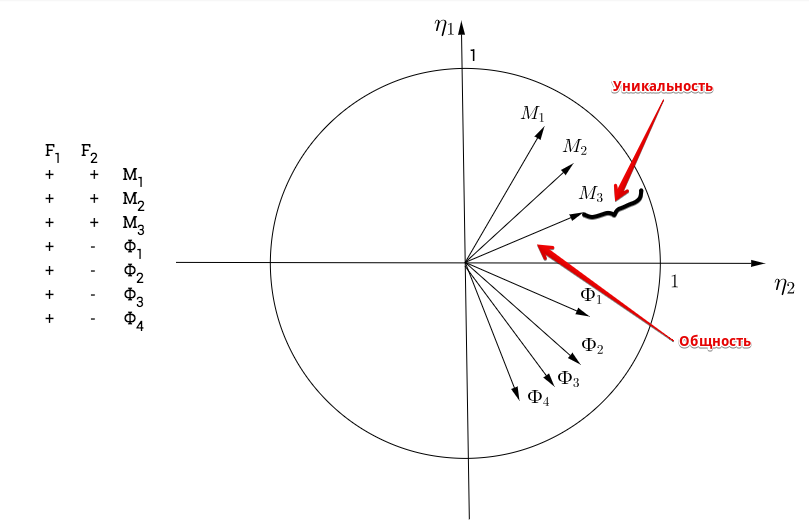
\includegraphics[scale=0.65]{img/Example.png}
	 \end{figure}
	
	
	При повороте осей примерно на $45^{\circ}$ получим скрытые факторы --- это способности по математике и по физике.
	
	{\bf{Не нашла материла про то, какие факторы не находит факторый анализ.}}
\end{ex}

    \ifxetex 
    {\color{blue} Набирала Стася}
\subsection{Билет 47. Методы нахождения факторных значений: LS и WLS (метод Бартлетта)}
  Матрица наблюдений $\mathbb X \in M_{n, p}(\R)$ в факторном анализе представляется как 
  $$\mathbb X = \mathbb V \mathbb F^\mathrm T + \eps, \mathbb V \in M_{n, r}(\R), \mathbb F \in M_{p, r}(\R), \eps \in M_{n, p}(\R).$$
  Перепишем для $\mathbb Y = \mathbb X^\mathrm T, \mathbb W = \mathbb V^\mathrm T$ (матрица $\mathbb Y = \left[Y_1:\cdots:Y_n\right]$ содержит наблюдения в столбцах):
  $$\mathbb Y = \left(\mathbb V \mathbb F^\mathrm T+ \eps\right)^\mathrm T = \mathbb F \mathbb V ^\mathrm T + \eps^\mathrm T \implies \forall i\in 1\mathbin{:}n\; Y_i = \mathbb F W_i + \eps_i.$$
  \begin{equation}\label{eq::factor_scores_regression}
    \begin{pmatrix}x_{i1} \\ \vdots \\ x_{ip}\end{pmatrix} = \mathbb F \begin{pmatrix}w_{i1} \\ \vdots \\ w_{ir}\end{pmatrix} + \begin{pmatrix}\eps_{i1} \\ \vdots \\ \eps_{ip}\end{pmatrix}
  \end{equation}
  
  \subsubsection{Ordinary Least Squares}
    При наличии уже оцененной матрицы факторных нагрузок $\mathbb F$ выражение \ref{eq::factor_scores_regression} может быть рассмотрено как задача линейной регрессии $W_i = (V^\mathrm T)_i$ на $\mathbb F$. Тогда для каждого наблюдения $Y_i$ можно построить соответствующие значения факторов
    $$\hat{W_i} = \left(\mathbb F^\mathrm T \mathbb F\right)^{-1}\mathbb F^\mathrm T Y_i.$$
    Модель линейной регрессии работает в предположении о гомоскедастичности (одинаковой вариантивности) данных, т.е. что $\eps_{i1}, \ldots, \eps_{ip}$ --- i.i.d. Модель фактороного анализа делает более слабое предположение: $\left(\eps_{i1}, \ldots, \eps_{ip}\right) \sim N(0, \diag{\left(\sigma_1^2, \ldots, \sigma_p^2\right)})$, т.е. вариативность (степень уникальности в контексте факторного анализа) у разных наблюдений разная.
  
  \subsubsection{Weighted Least Squares (метод Бартлетта)}\footnote{Я не смогла найти публикации, где бы в явном виде был изложен именно этот <<самый простой>> вариант}
    Приведём наши данные к виду, в котором они бы удовлетворяли модели линейной регрессии. Так, если $\eps_i\sim N(0, \Psi), \Psi = \cov{\eps_i} = \diag{\left(\sigma_1^2, \ldots, \sigma_p^2\right)}, \Psi^{-1/2} = \diag{\left(\frac{1}{\sigma_1}, \ldots, \frac{1}{\sigma_p}\right)}$, то 
    $$\cov{\left(\Psi^{-1/2}\eps_i\right)} = \Psi^{-1/2}\Psi\Psi^{-1/2} = \I_{p\times p} \implies \Psi^{-1/2}\eps_i \sim N(0, \I_{p\times p})$$
    Перепишем уравнение модели ФА так, чтобы уникальности в нём были вида $\Psi^{-1/2}\eps_i$:
    \begin{equation}
    \Psi^{-1/2} Y_i = \Psi^{-1/2} \mathbb F W_i + \Psi^{-1/2}\eps_i \iaoi \Psi^{-1/2} Y_i = \left(\mathbb F^\mathrm T \Psi^{-1/2}\right)^\mathrm T W_i + \Psi^{-1/2}\eps_i,
    \end{equation}
    тогда соответствующее выражение для оценки $W_i$ по МНК имеет вид
    $$\hat{W_i} = \left(\mathbb F^\mathrm T \Psi^{-1/2} \Psi^{-1/2} \mathbb F\right)^{-1}\mathbb F^\mathrm T \Psi^{-1/2}\Psi^{-1/2} Y_i = \left(\mathbb F^\mathrm T \Psi^{-1} \mathbb F\right)^{-1} \mathbb F^\mathrm T \Psi^{-1} Y_i.$$

    \subsection{Билет 48. Factor structure и factor pattern в случае ортогональных и неортогональных векторов}
	\begin{dfn}
		\emph{Factor structure} --- корреляции исходных признаков с факторами, $\cov{\left(\xi, \eta\right)}$.
	\end{dfn}
	\begin{dfn}
		\emph{Factor pattern} --- коэффициенты выражения исходных признаков через факторы.
	\end{dfn}

	Модель факторного анализа: $\xi = \mathbb F \eta + \eps, \cov{\eta} = I_{r\times r}$. Любое вращение с матрицей вращения $\mathbb W$ выражается как $\xi = \mathbb F \mathbb W^{-1} \mathbb W \eta + \eps = \mathbb F' \eta', \mathbb W \in M_r(\R)$. Тогда
	$$\cov{\eta'} = \cov{\mathbb W \eta} = \mathbb W \cov{\eta} \mathbb W^\T = \mathbb W \mathbb W^\T $$

	\danger{$\mathbb W \mathbb W^\T \not = I_{r\times r}$, так как для неортогональных вращений $\mathbb W^\T \not = \mathbb W^{-1}$.}

	Посчитаем factor structure:

	\begin{align*}
		\cov{\left(\xi,\eta'\right)} &= \cov{\left(\mathbb F' \eta' + \eps, \eta'\right)} = \cov{\left(\mathbb F' \eta', \eta'\right)} + \cov{\left(\eps, \mathbb W \eta\right)} =\\
		&= \mathbb F' \cov{\eta'} + 0 = \mathbb F' \mathbb W \mathbb W^\T = \mathbb F \mathbb W^\T.
	\end{align*}

	Если вращение было ортогональным, то $\mathbb W \mathbb W^\T = \mathbb W \mathbb W^{-1} = I$ и $\cov{\left(\xi,\eta'\right)} = \mathbb F$.

	Factor structure --- выражения исходных признаков через факторы, выписывается по определению модели:

	$$\xi_i = f_{i1}'\eta_{i1}' + \cdots + f_{ir}'\eta_{ir}' + \eps_i$$

	Следовательно, матрица коэффициентов линейной комбинации выражения исходных признаков через факторы --- это просто $\mathbb F'$.



    \else 
    \fi
\end{document}
